\usetikzlibrary{calc}
\tikzset{
    stackBox/.style={very thick},
    onStack/.style={thick},
}
\begin{frame}[fragile,label=vulnUAF]{vulnerable code}
\lstset{
    language=C++,
    style=smaller,
    moredelim={**[is][\btHL<2|handout:0>]{~2~}{~end~}},
}
\begin{tikzpicture}
\node[anchor=north east] (code) at (-1,0) {
\begin{lstlisting}
class Foo {
    ...
};
Foo *the_foo;
the_foo = new Foo;
...
delete the_foo;
...
something_else = new Bar(...);
the_foo->something();
\end{lstlisting}
};
\node[draw,anchor=north west,align=left] at (-3,0) {
    {\tt something\_else} likely where {\tt the\_foo} was
};
\begin{visibleenv}<2>
\draw[stackBox] (0, -2) rectangle (3, -5);
\draw[stackBox] (4, -2) rectangle (7, -5);
\draw[onStack,fill=blue!20] (0, -2) rectangle (3, -3) node[midway,align=center,font=\small] { vtable ptr (Foo) };
\draw[onStack,fill=blue!20] (0, -3) rectangle (3, -5) node[midway,align=center,font=\small] {data for Foo };
\draw[onStack,fill=yellow!20] (4, -2) rectangle (7, -3) node[midway,align=center,font=\small] { vtable ptr (Bar)? \\
                                                                                   other data? };
\draw[onStack,fill=yellow!20] (4, -3) rectangle (7, -5) node[midway,align=center,font=\small] { data for Bar  };
\end{visibleenv}
\end{tikzpicture}
\end{frame}

\begin{frame}{realistic use-after-free}
    \begin{itemize}
    \item code shown above seems very contrived
    \item though bugs that are this simple do happen
        \begin{itemize}
        \item usually immediate reuse does not cause problems
        \end{itemize}
    \vspace{.5cm}
    \item one likely case: two pointers to value
        \begin{itemize}
        \item example: object referenced from webpage + local variables in javascript
        \item example: object freed from one thread while another uses it
        \item example: ``reference count'' bookkeeping error
        \end{itemize}
    \item neglecting to handle case
    \end{itemize}
\end{frame}

\begin{frame}
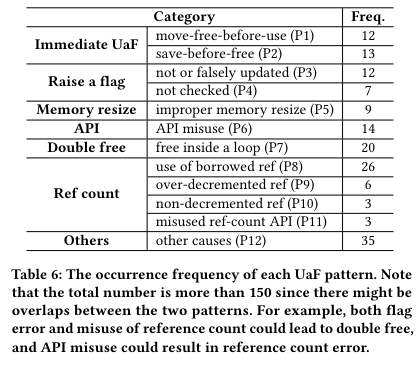
\includegraphics[height=0.8\textheight]{../uaf/uaf-causes-raid}
\imagecredit{Chen, Liu, Xiao, and Wang, ``All Use-After-Free Vulnerabilities are not Created Equal: An Empirical Study on Their Characteristics and Detectability'' (2023)}
\end{frame}

\begin{frame}
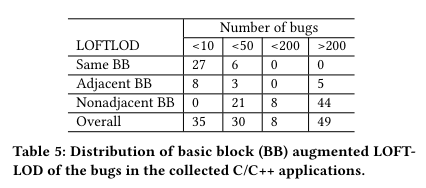
\includegraphics[height=0.7\textheight]{../uaf/uaf-distance} \\
(LOFTLOD = line of free to line of dereference; BB = basic block)
\imagecredit{Chen, Liu, Xiao, and Wang, ``All Use-After-Free Vulnerabilities are not Created Equal: An Empirical Study on Their Characteristics and Detectability'' (2023)}
\end{frame}

